\documentclass[a4paper,11pt,twoside]{scrartcl}
\usepackage[T1]{fontenc}
\usepackage{subcaption}
\usepackage[utf8]{inputenc}
\usepackage{ngerman, eucal, mathrsfs, amsfonts, bbm, amsmath, amssymb, stmaryrd,graphicx, array, geometry, color, wrapfig, float, hyperref}
\geometry{left=25mm, right=15mm, bottom=25mm}
\setlength{\parindent}{0em} 
\setlength{\headheight}{0em} 
\title{Machine Learning\\ Blatt 8}
\author{Markus Vieth\and David Klopp\and Christian Stricker}
\date{\today}
\usepackage{listings, textcomp}
\usepackage[usenames,dvipsnames,svgnames,table]{xcolor}


\definecolor{Code}{rgb}{0,0,0}
\definecolor{Keywords}{rgb}{0,0,255}
\definecolor{Strings}{rgb}{255,0,0}
\colorlet{Comments}{Green}
\colorlet{Numbers}{blue}

%%%%%%%%%%%
%Mache Integer farbig
%%%%%%%%%%%

\makeatletter

\newif\iffirstchar\firstchartrue
\newif\ifstartedbyadigit

\newcommand\processletter
{%
	\ifnum\lst@mode=\lst@Pmode%
	\iffirstchar%
	\global\startedbyadigitfalse%
	\fi
	\global\firstcharfalse%
	\fi
}

\newcommand\processdigit
{%
	\ifnum\lst@mode=\lst@Pmode%
	\iffirstchar%
	\global\startedbyadigittrue%
	\fi
	\global\firstcharfalse%
	\fi
}

\lst@AddToHook{Output}%
{%
	\ifstartedbyadigit%
	\def\lst@thestyle{\color{Numbers}}%
	\fi
	\global\firstchartrue%
	\global\startedbyadigitfalse%
}

\newtoks\jubo@toks
\jubo@toks={
	language=C,
	commentstyle=\color{Comments}\slshape,
	stringstyle=\color{Strings},
	keywordstyle={\color{Keywords}\bfseries},
	alsoletter=0123456789,
	SelectCharTable=%
}
\def\add@savedef#1#2{%
	\begingroup\lccode`?=#1\relax
	\lowercase{\endgroup
		\edef\@temp{%
			\noexpand\lst@DefSaveDef{\number#1}%
			\expandafter\noexpand\csname lsts@?\endcsname{%
				\expandafter\noexpand\csname lsts@?\endcsname\noexpand#2}%
		}}%
		\jubo@toks=\expandafter{\the\expandafter\jubo@toks\@temp}%
	}
	\count@=`0
	\loop
	\add@savedef\count@\processdigit
	\ifnum\count@<`9
	\advance\count@\@ne
	\repeat
	\count@=`A
	\loop
	\add@savedef\count@\processletter
	\ifnum\count@<`Z
	\advance\count@\@ne
	\repeat
	\count@=`a
	\loop
	\add@savedef\count@\processletter
	\ifnum\count@<`z
	\advance\count@\@ne
	\repeat
	%\showthe\jubo@toks % for debugging
	\begingroup\edef\x{\endgroup
		\noexpand\lstdefinestyle{pseudo}{\the\jubo@toks}
	}\x
	
	\makeatother
%%%%%%%%%%
%Ende
%%%%%%%%%%



\lstset{
	literate={ö}{{\"o}}1
	{ä}{{\"a}}1
	{ü}{{\"u}}1
	{ß}{{\ss}}1
	{/pi}{{$\Pi$}}1
	{/inf}{{$\infty$}}1
	{/eIn}{{$\in$}}1
	{/cup}{{$\cup$}}1
	{/leer}{{$\emptyset$}}1
	{<=}{{$\leq$}}1
	{>=}{{$\geq$}}1
}


\lstset{
	numberstyle=\tiny,
	stepnumber=1,
	numbersep=10pt,
	xleftmargin=15pt,
	breaklines=true,
	numberblanklines=false,
	showstringspaces=false,
	flexiblecolumns=true,
	mathescape=true,
	tabsize=4,
	captionpos=b,
	numbers=left,
	commentstyle=\color{Green},
	numberstyle=\color{gray},
	keywordstyle=\color{blue} \textbf,%otherkeywords={xdata},
	keywords=[2]{xdata},
	keywordstyle=[2]\color{red}\textbf,
	identifierstyle=\color{black},
	stringstyle=\color{red}\ttfamily,
	basicstyle = \ttfamily \color{black} \footnotesize,
	inputencoding=utf8,
	emph=[1]%
	{%
		infinity,
	}, 
	emphstyle=[1]{\color{blue}},
	emph=[2]%
	{%
		forall,
		while,
		if,
		else,
		for,
		return,
		new,
		NULL,
		null,
		int, 
		double, 
		float,
		class,
		void,
		false, 
		true,
		FALSE,
		TRUE,
	}, 
	emphstyle=[2]{\color{Magenta}},
	emph=[3]{b0, b1, n0, n1},
	emphstyle=[3]{\color{black}}
}
\begin{document}

\newcommand{\cor}[1]{\textcolor{red}{\textit{#1}}}
\maketitle
\cleardoublepage
\pagestyle{myheadings}
\markboth{Markus Vieth,  David Klopp, Christian Stricker}{Markus Vieth, David Klopp, Christian Stricker}

\section*{Curse of Dimensionality}

The nearest neighbor method breaks in high-dimensional spaces, because the ''neighborhood'' becomes very large for the Euclidean distance. This is called the curse of dimensionality. Suppose  we have 5000 points uniformly distributed in the n-dimensional unit hypercube $C_n := [0,1]^n$ and we want to apply the 5-nearest neighbor algorithm. Suppose our query point is at the origin $(0, \ldots, 0)$, so, on average, we need to search $5/5000$ of the hypercube's volume to capture the 5 nearest points.

\paragraph*{1.} Assume$ n=2, i.e. C_n$ is the unit square. What is the side length d of the square $[0,d]^2$ that on average captures the five nearest points to the origin?

\begin{figure}[H]
\center
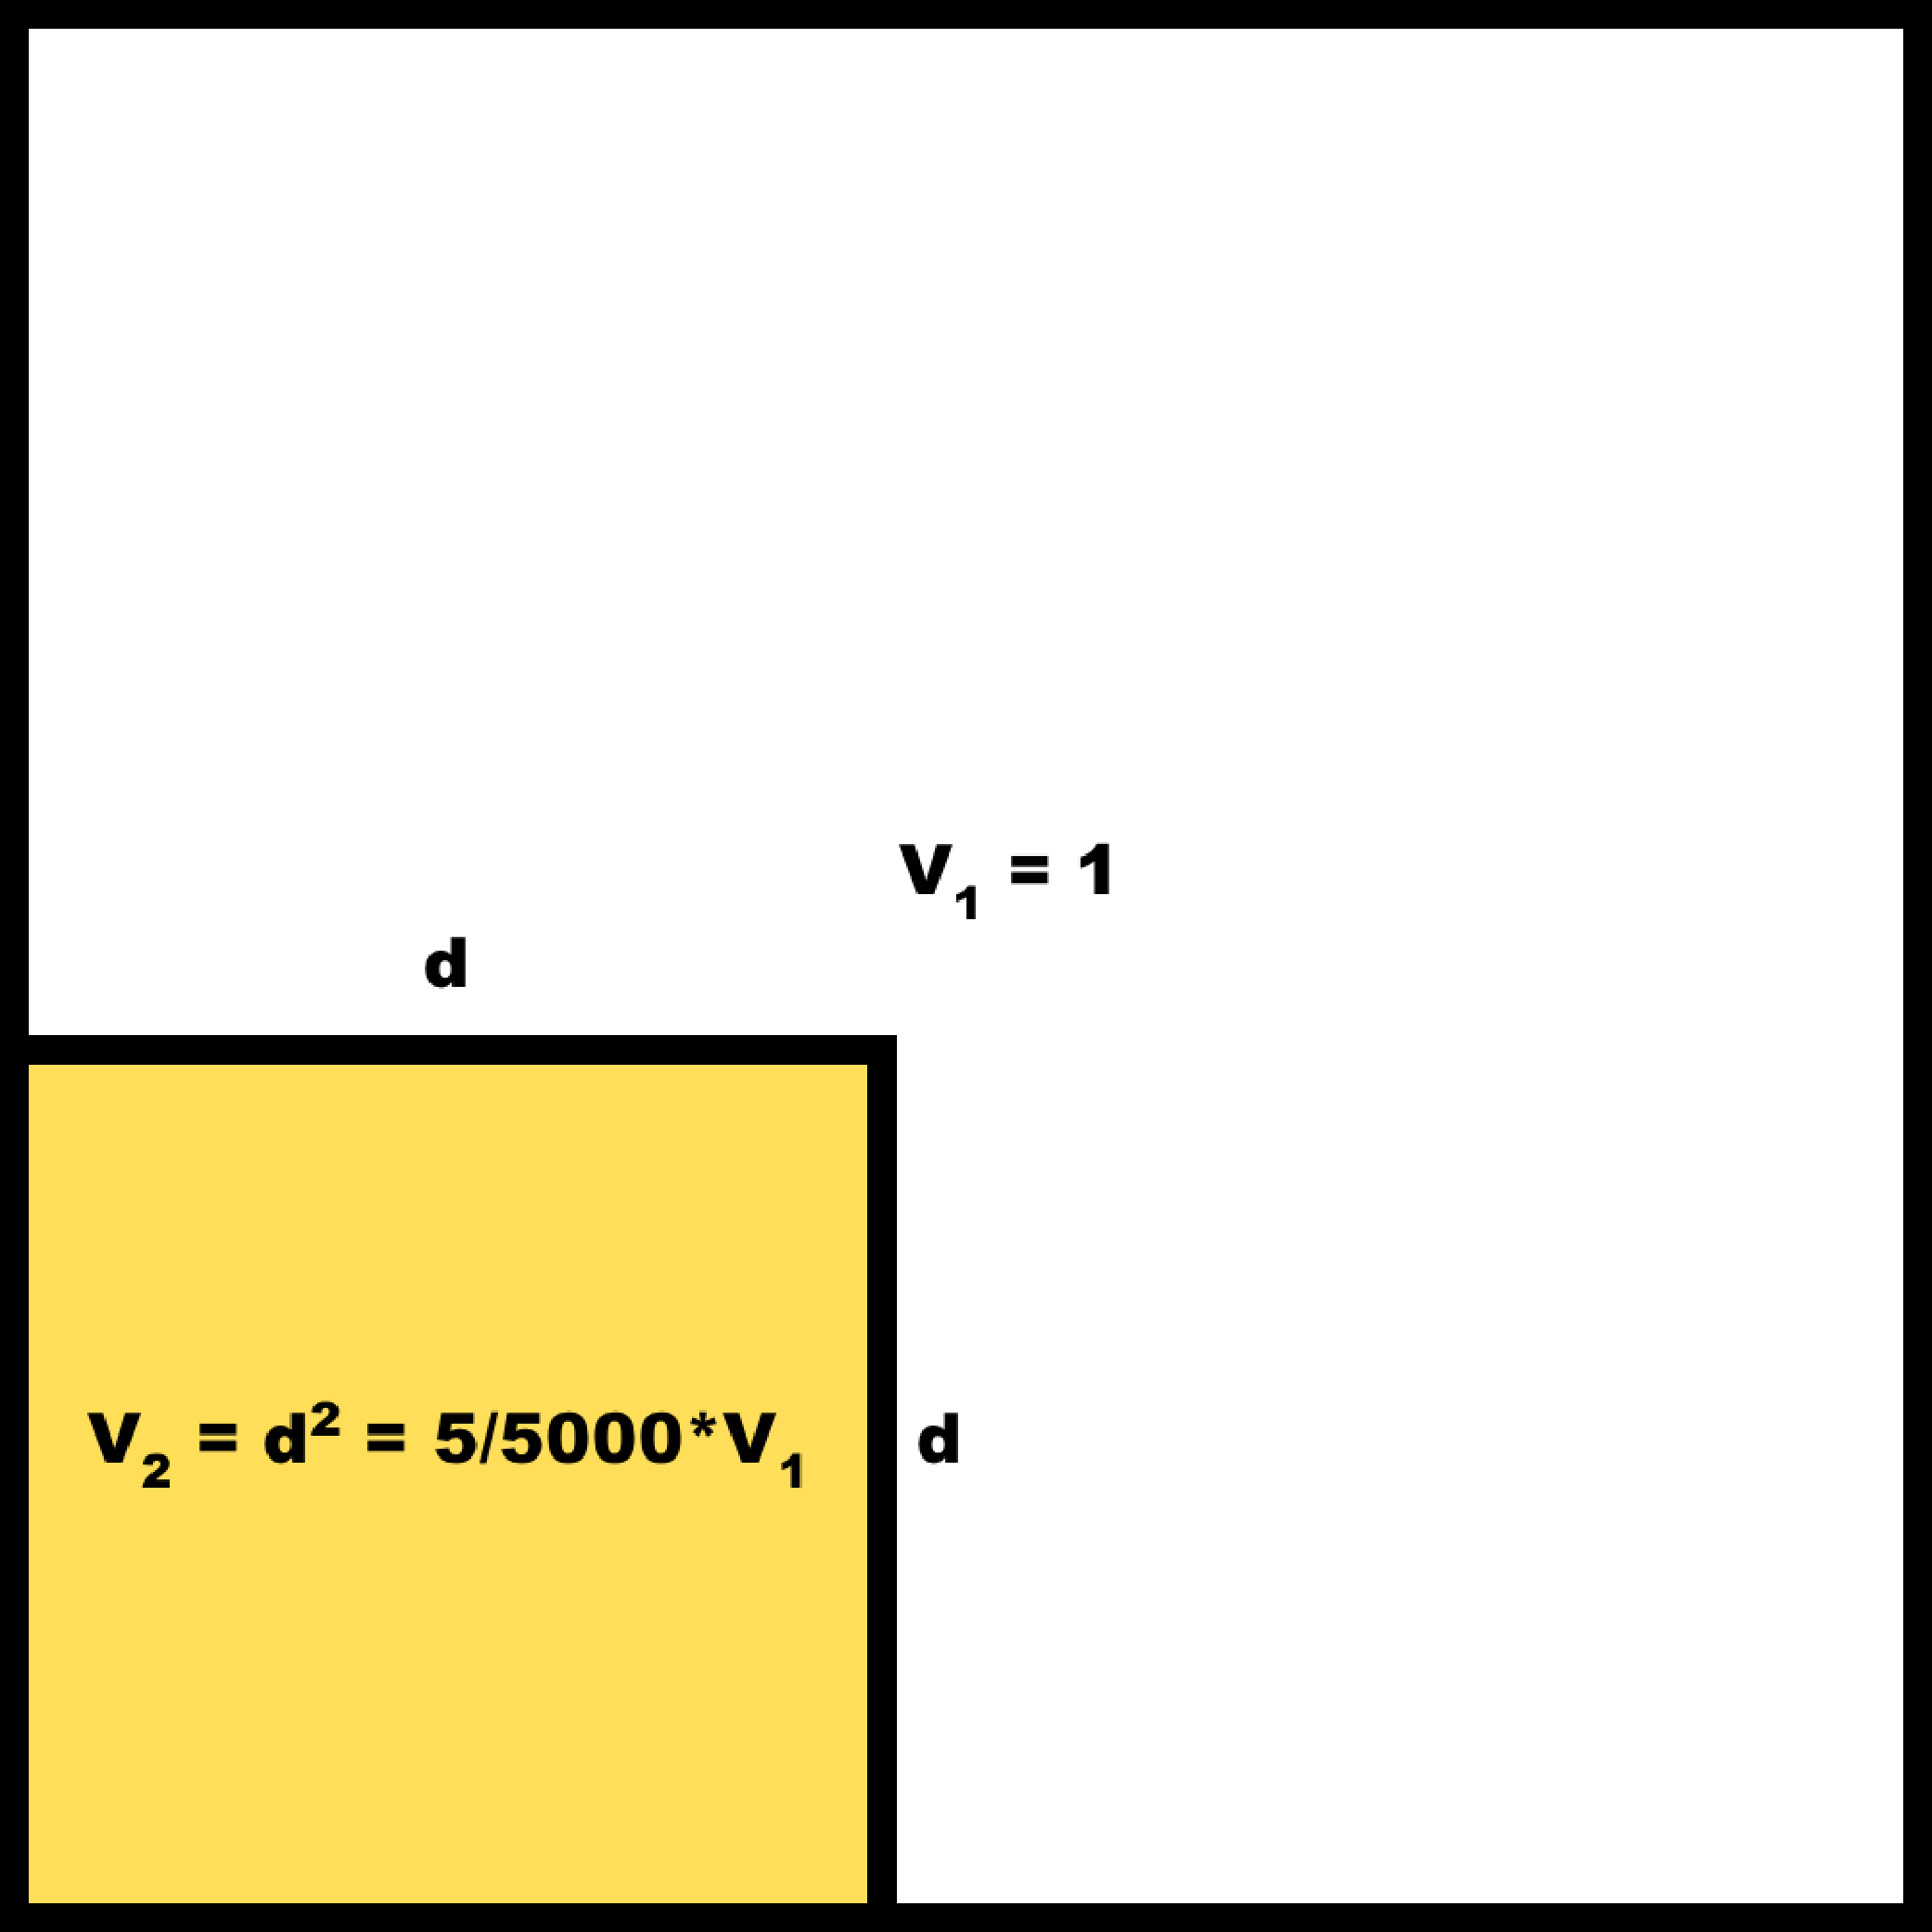
\includegraphics[width=0.3\textwidth]{images/1_1.pdf}
\end{figure}

\[d^2 = \frac{5}{5000} \]
\[\Leftrightarrow d = \sqrt{\frac{5}{5000}} = \sqrt{\frac{1}{1000}} = \sqrt{\frac{1}{10 \cdot 100}} = {\frac{1}{\sqrt{10} \cdot 10}} = {\frac{\sqrt{10}}{100}}\]

\paragraph*{2.} What is the side length d of the n-dimensional hypercube $[0,d]^n$ that on average captures the five nearest points to the origin?
\[d^{\:n} = \frac{5}{5000} \]
\[\Leftrightarrow d = \sqrt[n]{\frac{1}{1000}} = 1000^{-\frac{1}{n}}\]

\paragraph*{3.}  For which number of dimensions n do we need a hypercube $[0,d]^n$ whose side length is larger than half  the side length of $C_n$ (i.e. 0.5) to capture the five nearest points?

\[d \geq 0.5 \]
\[\Leftrightarrow d^{\:n} \geq 0.5^n = d^{\:n} \geq 2^{-n}  \]
\[\Leftrightarrow \frac{1}{1000} \geq 2^{-n} \]
\[\Leftrightarrow \log_2{\left(\frac{1}{1000}\right)} \geq \log_2{(2^{-n})} \]
\[\Leftrightarrow \log_2{\left(1000^{-1}\right)} \geq -n \cdot \log_2{2} \]
\[\Leftrightarrow \log_2{\left(1000\right)} \leq n \]
\[\Leftrightarrow n \geq 10 \]

\pagebreak

\section*{Voronoi Diagram}

A two-dimensional data set contains the five points (1,2), (3,1), (6,3), (3,4), and (2,6).
\paragraph*{1.} Draw the Voronoi diagram for this data set.
\begin{figure}[H]
\center
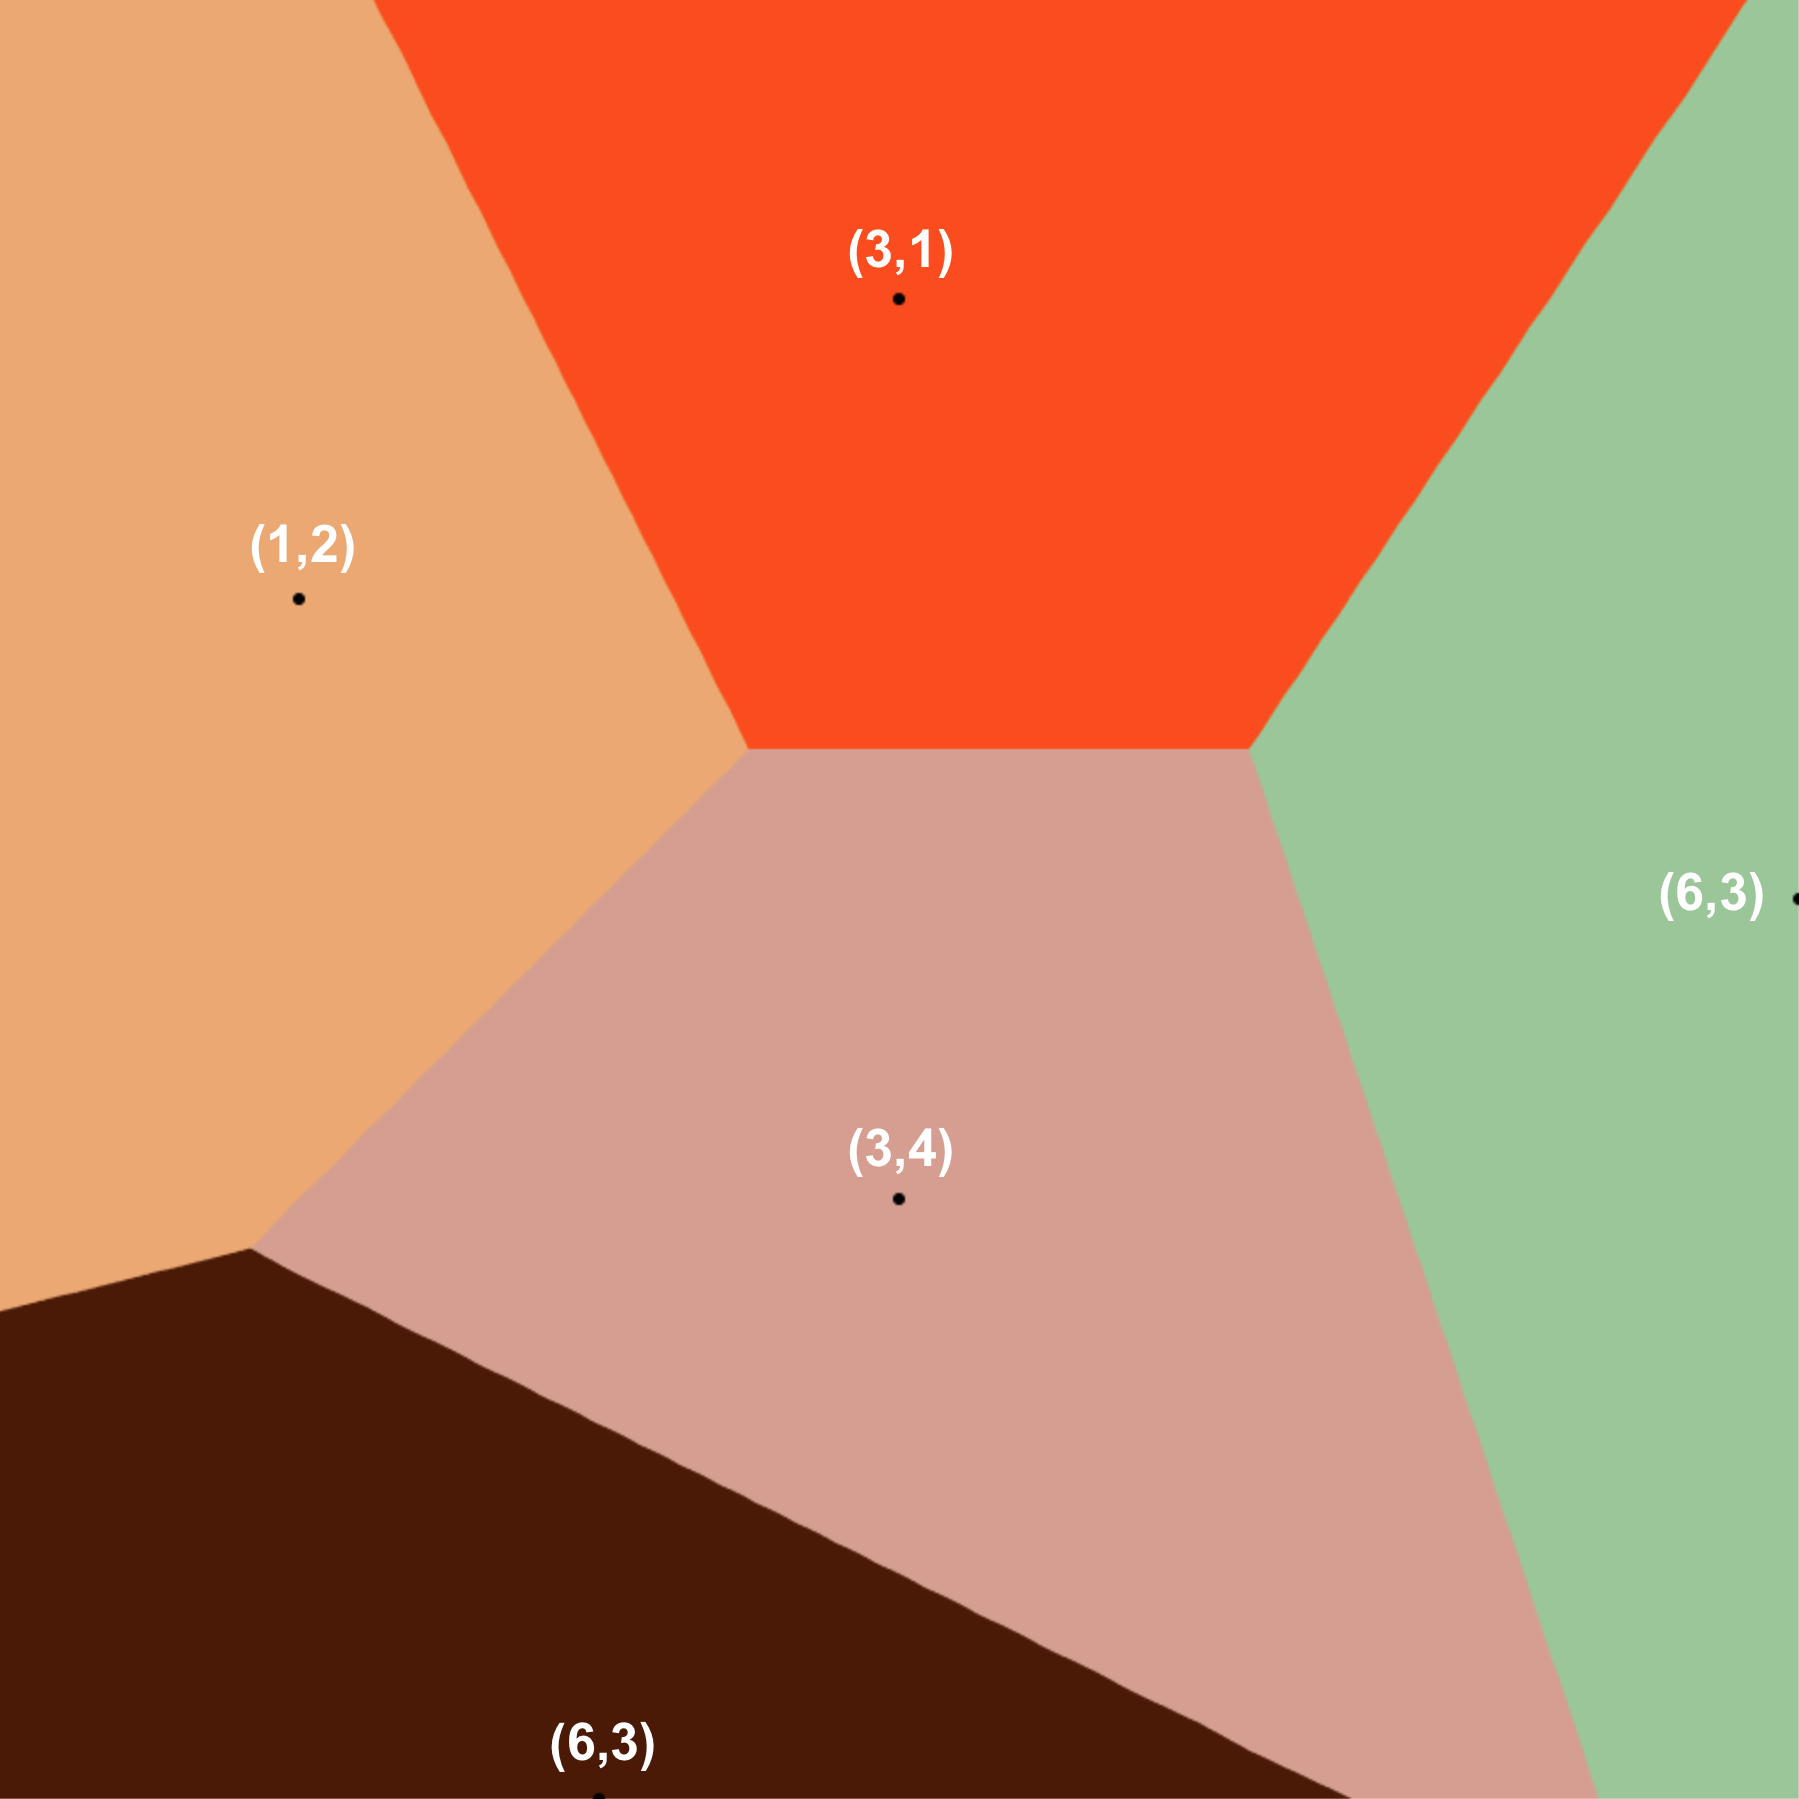
\includegraphics[width=0.6\textwidth]{images/voronoi_diagram.png}
\end{figure}



\paragraph*{2.} Why is it impractical to store the Voronoi diagram in order to speed up queries for $k$-nearest neighbor? (Two sentences) \\

Die Zuordnung eines Punktes zu einer bestimmten Nearest Neighbour Suchregion kann in einem Voronoi Diagram nicht effizient realisiert werden. Es resultiert also kein wirklicher Zeitgewinn in der Speicherung von Voronoi Diagrammen.

\end{document}